\chapter{Multilingual Data and Machine Translation}
\label{ch:mt}

So far, we have been focusing on monolingual topic models and their applications.
But many collections contain documents in more than one language.
In practice, we often discover this phenomenon unexpectedly after running an initial monolingual topic model: topic models turn out to be very good at language identification.
This behavior makes sense because the model is looking for groups of words that appear frequently together but not in other contexts, and separate languages will exhibit this property strongly.
In some cases we may choose to filter out small numbers of documents in other languages, but in many cases we would like to take advantage of  connections across many languages.

Multilingual topic models have been developed to analyze and understand a corpus in multiple languages.
\citet{vulic2015probabilistic} provide a good overview.
The applications in multi-language corpora can be divided into two categories.
The first, and simpler category is those that align languages at the topical level, but not at the level of individual word types.
These models are useful for organizing corpora, but make no attempt to support analysis for users unfamiliar with any particular language.
The second category is those that explicitly model word-level alignments across languages.
These models support applications in statistical machine translation~(\textsc{smt}).

As one of the most frequent applications for multilingual topic models, \textsc{smt} tries
to find a sequence of words in one language  which match the meaning of a text input
in another language. While the training data of \textsc{smt} requires explicit aligned sentences
in different languages, multilingual topic models relax this data restriction and are flexible to 
explore only loosely aligned data.  In this chapter, we first discuss how topic models are 
adapted to use multiple languages, and then show how these multilingual topic models can 
help \textsc{smt}.

Before discussing specific methods, it is useful to define terms related to data sources.
The most salient feature for multilingual corpora is their degree of alignment.
Parallel corpora are the most closely aligned. These collections comprise subsets of documents such that each set contains documents in different languages that have the same semantic content (up to the limits of translation).
Common examples include translations of literary works or translated government documents, where a transcript of a speech in French is accompanied by a transcript of the  same speech in German, with as little semantic difference as possible.
Comparable corpora are less closely aligned. 
These collections also contain subsets of documents, but each set is only constrained to be {\em topically} similar, and not necessarily a direct translation.
A common example is articles in Wikipedia.
The articles for the French city of Lille in English and French Wikipedia are referring to the same place and contain much of the same information, but the French version is considerably longer.
Mixed corpora are the least aligned. These collections simply contain documents in more than one language, but there is not necessarily any connection between any one document in one language and a document in another language.
An example might be a journal that publishes in English, French, German, and Italian.
No article is a translation of any other article.
There are likely to be topical overlaps between articles, but there are not necessarily any structural indications of such relationships.
A last category of useful data, not necessarily in the form of documents, is a bilingual lexicon that maps words in one language to words in another.
Lexicons of this form can be considered to be examples of parallel corpora with single-token documents, but it is often useful to treat them specially.

\section{Document-level Alignment from Multilingual Corpora}
\label{sec:doc-align}

In a case where a user is browsing a multilingual collection with only monolingual knowledge
to find relevant documents, multilingual topic models can help. Such collections contain
multiple languages, but does not necessarily have the exact matching or translations 
on words and sentences. Only a coarse document alignment is necessary, as long as the documents
discuss the same topics, e.g., Wikipedia articles in different
languages. Such connection between languages is also helpful to infer
more robust topics, since different languages can complement each
other to reduce ambiguity.

This approach pre-dates probabilistic topic models.
\citet{Landauer-1990} connect aligned documents in different languages
by projecting both documents to a shared latent semantic indexing
space.

Similarly, bilingual topic models~\citep{zhao-06,DeSmet-09} and polylingual topic models~\citep{mimno-09}
such as polylingual Latent Dirichlet Allocation~(\plda{})
assume that the aligned documents in different languages share the
same topic distribution and each language has a unique topic
distribution over its word types.
Thus the generative process of polylingual topic model is as follows:
given a document pair $(d_{l_1}, d_{l_2})$, we first sample a
document-topic distribution $\theta_d$; for a document $d_{l_i}$ in
language $l_i$, we then sample a topic $z_{dn}$ from $\theta_d$, and
generate a word from topic $\phi_{z_{dn}, l_i}$ in language $l_i$.

Topic models trained from document-level alignments have applications in exploratory data analysis and in information retrieval \citep{vulic2013cross}.
\citet{mimno-09} use a model trained on multiple languages in Wikipedia to compare relative interest in different topics across linguistic domains.
For example, the Persian-language Wikipedia has a larger than average number of articles about science, while the Finnish-language Wikipedia has a larger than average number of articles about skiing.
These methods require parallel or comparable corpora, but for mixed corpora the training data can be augmented with a supplemental corpus of comparable documents as long as  the comparable documents cover similar enough topics \citep{mimno-12b}.

We note that it is not necessary to take ``language'' in its strict meaning.
Loosely aligned models have been applied in information retrieval for query expansion \citep{Gao-2011,Gao-2012}. 
While the topic models' application in information retrieval (Chapter~\ref{ch:ir}) focus
on a single language, \cite{Gao-2011} assume the queries and Web documents are in
different ``languages''. The query language from users are normally informal oral language, 
which are less formatted and may include abbreviation as well. However, the document language
are more formal and well organized written language. For example, given a query ``dtd amc'',
the relevant Web document may contain ``downtown disney amc''~\citep{Jiang-2016}. 

This semantic gap~\citep{Muller-2009} between queries and documents
provides the possibility to treat queries and documents as different languages, and the relevance between
queries and documents make them loosely aligned. Based on this assumption, 
they further assume queries and documents share the same document-topic
distributions $\theta^Q$, but have different topic-word distributions
$\phi_z^Q$ and $\phi_z^D$ respectively.
%To generate a query $q$, a document-topic distribution $\theta^Q$ is
%drawn from a Dirichlet prior, and a topic $z$ is sampled from
%$\theta^Q$, then a query term $q_i$ is sampled from $\phi_z^Q$. To
%generate a document term, a topic $z$ is firstly sampled from
%$\theta^Q$, the same document-topic distribution as the query, and
%then a document term $d_i$ is sampled from document topic-word distribution $\phi_z^D$. 
In this way, documents and queries are
connected through the hidden topics, even though their vocabularies
(topic-word distributions) are different. By summing over all possible
topics, the relationship between document term $e$ and query $q$ is
\begin{align}
p(e \g q) = \sum_k p(e \g \phi_k^D) p(k \g \theta_q).
\end{align}

%\jbgcomment{Would be good to have an example of this soft query \yhcomment{David added this example, and I don't actually understand what he means here.}}

Some forms of query expansion across multiple languages do not require
explicit modeling of connections between topics \citep{vulic2011crosslanguage,vulic2015probabilistic}.  As noted in
Chapter~\ref{ch:ir}, \citet{erlin2017topic} use two independent seeded
models on English and German books to search for works about
epistemology.  After manually identifying one \underline{epistemology}
topic from each language's model, these two topics are used as a form
of query expansion to identify documents related to the target
subject.

Although it is relatively easy to get comparable topics from comparable corpora, identifying specific words that are translations of each other in different languages is more difficult.
Given a word $w_e$ that has high probability in topic $k$ in language $e$, it is likely that a good translation of $w_e$ in language $f$ has high probability in topic $k$ as well. \citet{vulic2011identifying} evaluate several methods for identifying such translation pairs given a bilingual or polylingual topic model.
They find two methods that work well, both of which consider the frequency of a given target word across many topics.
The intuition is that words that have high probability in a given topic because they are specific to that topic are more likely to be good translations than words that have high probability in a topic because they are frequent in the corpus overall, and are thus represented in many topics.
The authors were then able to derive an algorithm for finding high-quality aligned translation pairs \citep{vulic2012detecting}. This method is capable of using word patterns as hints for etymologically related words when available, but is also effective even for unrelated languages.
However, there are limits to our ability to find direct translation pairs with only document-level alignment, both because the data is not sufficient, and because languages may align more at the level of {\em concepts} rather than specific lexical items \citep{vulic2014probabilistic}.

\section{Word-level Alignment from Lexical Data}

Aligned documents are useful when a collection is designed to be
lightly multilingual: e.g., when the creators are building a
native-language version of Wikipedia.  Documents links
are cheap and easy. However, they require active support of those creating the
collection, which is not always available.  Many collections are
written in isolation.

However, one of the most ubiquitous multilingual tools is the
dictionary.  This section discusses how we can use \emph{lexical information} like
multilingual dictionaries~\citep{Zhang-10} and orthographic relations 
between words~\citep{boyd-graber-09} to help users
who want to understand a collection.

For instance, tree-based topic models such as tree-based Latent Dirichlet 
Allocation~(\abr{tlda})~\citep{boyd-graber-07,andrzejewski-09,hu-14:itm}
incorporate positive correlations between words in the same or
different languages by encouraging words that appear together in a
{\bf concept} to have similar probabilities given a
topic.\footnote{\citet{Zhang-10} use
  topic-level soft constraints to achieve a similar effect.} These
concepts can come from WordNet~\citep{boyd-graber-10}, domain
experts~\citep{andrzejewski-09}, or user
constraints~\citep{hu-14:itm}. If these concepts are in the same
language, the backend model is the same as monolingual interactive topic modeling
introduced in Chapter~\ref{ch:viz}. However, when we gather concepts
from bilingual resources, these concepts can connect different
languages. For example, if a bilingual dictionary defines
``\begin{CJK*}{UTF8}{gbsn}电脑\end{CJK*}'' as ``computer'', we combine
  these words in a concept.

  These concepts (positive correlations) are organized into a {\bf
    prior tree} structure. Words in the same concept share a common
  parent node (Figure~\ref{fig:prior_trees}). That concept then
  becomes one of many children of the root node.  Words that are not
  in any concept---{\bf uncorrelated words}---are directly connected
  to the root node. Thus a topic becomes a distribution over all paths
  in this prior tree and each path is associated with a word.

\begin{figure}
\centering
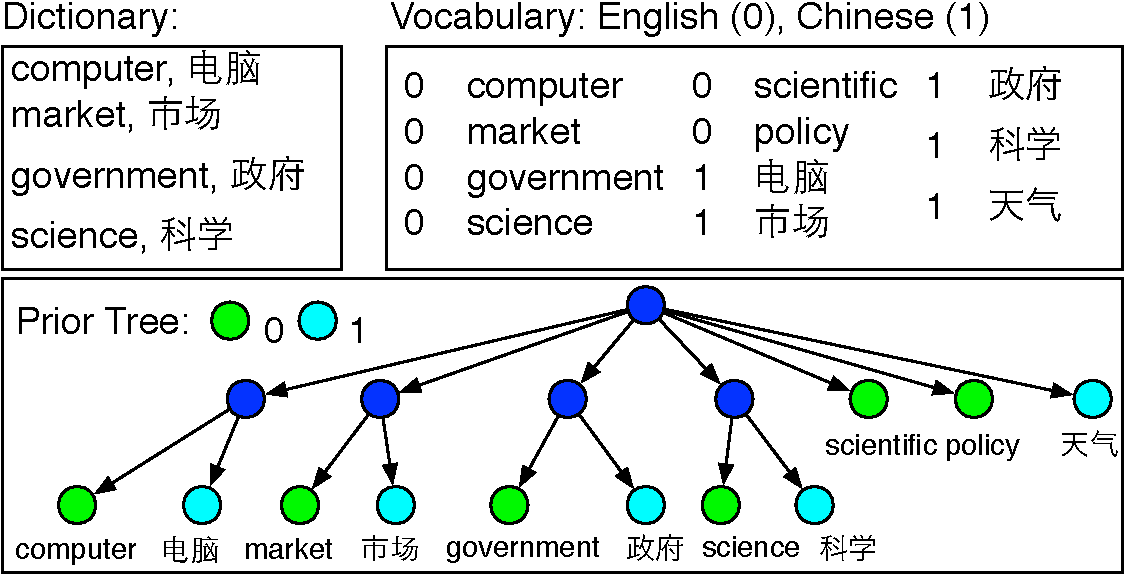
\includegraphics[width=0.9\linewidth]{figures/correlations_tree-crop.pdf}
\vspace{-3mm}
\caption[Constructing prior tree from a bilingual dictionary]{An example of constructing a prior tree from a
  bilingual dictionary: word pairs with the same meaning but in
  different languages are concepts; a common parent node is created to
  group words in a concept, and then is connected to the root;
  uncorrelated words are connected to the root directly.}
\label{fig:prior_trees}
\end{figure}

The probability of a path in a topic depends on the transition
probabilities in a topic.  Each concept $i$ in topic $k$ has a
distribution over its child nodes that is governed by a Dirichlet prior:
$\pi_{k,i} \sim \text{Dir}(\beta_{i})$.  Each path ends in a word
(i.e., a leaf node) and the probability of a path is the product of
all of the transitions between topics it traverses. Topics have
correlations over words because the Dirichlet parameters can encode
positive or negative correlations~\citep{andrzejewski-09}.

As a result, to sample a word $w_{dn}$ given a topic $z_{dn}$, a path
$y_{dn}$ from the topic tree of topic $z_{dn}$ is sampled: we start
from the root $n_0$ and first sample a child node $n_1$ of the root;
if node $n_1$ is a concept node, we continue to sample a word node
$n_2$ and generate the word associated with $n_2$; if node $n_1$ is a
word node already, we generate the word directly.

When this tree serves as a prior for topic models, words in the same
concept are positively correlated in topics.  For example, if
``\begin{CJK*}{UTF8}{gbsn}电脑\end{CJK*}'' has high probability in a
  topic, so will ``computer'', since they share the same parent
  node. With the tree priors, each topic is no longer a distribution
  over word types; instead, it is a distribution over paths, and each
  path is associated with a word type.  The same word could appear in
  multiple paths, and each path represents a unique sense of this
  word.

\section{Alignment from Parallel Corpora and Lexical Information}

Bilingual dictionaries and other sources of word-level information are 
valuable in training multilingual models, because they can easily specify 
simple lexical relationships that might be difficult to extract from parallel corpora.
But such manually generated data may be brittle, low-quality, or missing contextual differences in actual usage.
These two approaches are not mutually exclusive, however; they reveal
different connections across languages. \citet{hu-14} bring existing
tree-based Latent Dirichlet Allocation~(\tlda{}) and polylingual Latent Dirichlet 
Allocation~(\plda{}) together and create the polylingual tree-based Latent Dirichlet 
Allocation~(\ptlda{}) that incorporates both word-level correlations and
document-level alignment information.

To build up the prior tree structure, \citet{hu-14} consider two
resources that correlate words across languages. The first is
multilingual dictionaries, which match words with the same meaning in
different languages together. The other is the word alignments
extracted from aligned sentences in a parallel corpus. These relations
between words are used as the concepts~\citep{Bhattacharya-2006} in
the prior tree (Figure~\ref{fig:prior_trees}).

Given the prior tree structure, the generation of documents is a
combination of \tlda{} and \plda{}.  For each aligned document pair
$(d_{l_1}, d_{l_2})$, we first sample a distribution over topics
$\theta_d$ from a Dirichlet prior $\text{Dir}(\alpha)$.  For each
token in the aligned document $d_{l_i}$, we first sample a topic
$z_{dn}$ from the multinomial distribution $\theta_d$, and then sample
a path $y_{dn}$ along the tree of topic $z_{dn}$. Because every path
$y_{dn}$ leads to a word $w_{dn}$ in language $l_{dn}$, we append the
sampled word $w_{dn}$ to document $d_{l_{dn}}$ in language $l_{dn}$.

If we use a flat symmetric Dirichlet prior in place of the tree prior,
the model is equivalent to \plda{}. Similarly, if all documents are monolingual (i.e., with
distinct distributions over topics $\theta$), the model is equivalent to \tlda{}. \ptlda{} connects different languages on both the word
level (using the word correlations) and the document level (using the
document alignments), thus it learns better topics by considering more
information from both languages.



\section{Topic Models and Machine Translation}
\label{sec:tm-mt}

The most frequent application of multilingual topic models is in machine translation.
Given a text input in one language (source language), statistical
machine translation tries to find a similar sequence of words in another
language (target language). Modern machine translation
systems~\citep{koehn-09} use millions of training examples to learn
the translation rules and apply these rules on the test data. 
Topic models are useful in this application when they can help to inform word meaning and word choice in specific contexts.
While the translation rules are learned in local context, these systems work
best when the training corpus has a consistent \emph{domain}, such as a
 genre (e.g., sports, business) or style (e.g.,
newswire, blog-posts). 

Translations within one domain are better than translations across
domains since they vary dramatically in their word choices and style.
A correct translation in one domain may be inappropriate in another
domain.  For example, ``\begin{CJK*}{UTF8}{gbsn}潜水\end{CJK*}'' in the
  \underline{sports} domain usually means ``underwater diving'', but
  in the \underline{social media} domain, it means a non-contributing
  ``lurker''. To avoid such translation errors caused by domain
  shift, train translation must be robust to such systematic variation
  in the training set.  This is called \emph{domain adaptation}.

To train such \textsc{smt} systems, early
efforts focused on building separate models given the hand-labeled
domains~\citep{foster-07,matsoukas-09,chiang-11}. However, this setup
is at best expensive and at worst infeasible for large data.  Topic
models provide a promising solution where domains can be automatically
discovered. Each extracted topic is treated as a soft
domain.\footnote{Henceforth we will use the term ``topic'' and
  ``domain'' interchangeably: ``topic'' to refer to  a word distribution in
  topic models and ``domain'' to refer to \textsc{smt} corpora.} Thus
the normal monolingual topic models trained only on the source documents have
been applied to extract domain knowledge for machine
translation~\citep{Eidelman-12}.

However, the source language the and target language can complement
each other to build up more accurate topic models. For example, if we
only know the Chinese phrase ``\begin{CJK*}{UTF8}{gbsn}潜
  水\end{CJK*}'', it is hard to decide whether it is a
  \underline{sport} domain or it is a \underline{social media}
  domain. However, with the help of the aligned English translation
  ``lurker'', it is easy to identify the ``social media'' domain. Thus
  multilingual topic models~\citep{ni-09,DeSmet-09} have been
  applied to extract domain knowledge for machine
  translation~\citep{hu-14}.

\section{The Components of Statistical Machine Translation}

Statistical machine translation represents translation as a
combination of probabilistic processes, a phrase-level translation model and a sentence-level language model~\citep{koehn-03,koehn-09}. 
Topic models have been applied to both aspects of this process.

The actual process of translation is also known as \textit{decoding},
which is to find the best translation target sentence $\mathbf{e}$ 
given the source sentence $\mathbf{f}$. Formally,
Given a source sentence $\mathbf{f}$, the best
translation in target language $\mathbf{e}_\texttt{best}$ is
\begin{equation}
\mathbf{e}_\texttt{best} = \textbf{argmax}_\mathbf{e} p(\mathbf{e}|\mathbf{f}) = \textbf{argmax}_\mathbf{e} p(\mathbf{f}|\mathbf{e}) p (\mathbf{e}),
\end{equation}
which is split to a \textit{translation model}
$p(\mathbf{f}|\mathbf{e})$ and a \textit{language model} $p
(\mathbf{e})$.
Intuitively, a good translation should be both a good match for the source sentence (scoring high in the translation model) 
and a good sentence in its own right (scoring high in the language model).

In the \textit{decoding} phase, the source sentence $\mathbf{f}$ is segmented into multiple source
phrases $\bar{f}_n$, which are translated to a set
of target phrases $\bar{e}_n$. Thus the translation probability
$p(\mathbf{f}|\mathbf{e})$ can be further decomposed to the phrase
translation probability $p(\bar{f}_n | \bar{e}_n)$.
In the \textit{reordering} phase target phrases may then need to be repositioned to get the best
translation result. Reordering is captured by a relative distortion
probability distribution $d(a_n - b_{n-1})$, where $a_i$ denotes the
start position of the source phrase that was translated to the $n$\textsuperscript{th}
target phrase, and $b_{n-1}$ denotes the end position of the source
phrase translated into the $(n-1)$\textsuperscript{th} target phrase. As a result, the
translation model decomposes into
\begin{equation}
p(\mathbf{f} \g \mathbf{e}) = \prod_{n} p(\bar{f}_n \g \bar{e}_n) d(a_n - b_{n-1})
\end{equation}

In phrase-based \textsc{smt}, the phrase probability $p(\bar{f}_n \g
\bar{e}_n)$ can be further estimated by combining lexical translation
probabilities of words contained in that phrase~\citep{koehn-03},
which is normally referred as \textit{lexical weighting}. Lexical
conditional probabilities $p_w(f \g e)$ are maximum likelihood estimates
from relative lexical frequencies,
\begin{equation}
\label{eq:lexical_prob}
p_w(f \g e) = \textstyle \slfrac{c(f, e)}{\sum_f{c(f, e)}}
\end{equation}
where $c(f, e)$ is the count of observing lexical pair $(f, e)$ in the
training dataset. Given a word alignment $a$, the lexical weight for
this phrase pair $p_w(\bar{f} \g \bar{e}; a)$ is the normalized product
of lexical probabilities of the aligned word pairs within that phrase
pair:
\begin{equation}
\label{eq:phrase_prob}
p_w(\bar{f} \g \bar{e}; a) = \prod_{i} \frac{1}{\{|j \g (i, j) \in a\}|} \sum_{\forall (i,j) \in a} p_w(f_i \g e_j)
\end{equation}
where $i$ and $j$ are the word positions in target phrase $\bar{e}$
and source phrase $\bar{f}$ respectively.

Next we introduce how to apply topic models to improve translation
models, language models, and reordering models respectively.


\section{Topic Models for Phrase-level Translation}
\label{sec:trans-multiling}

Translation models map words and phrases from one language to another.
Both monolingual topic models and bilingual topic models are useful for improving translation models.
As we have mentioned in Section~\ref{sec:tm-mt}, 
the most prominent application of topic models is in {\em domain adaptation}.

Early work for extracting domain knowledge focus on the hand-labeled domains~\citep{foster-07,matsoukas-09,chiang-11}.
These labels are not only expensive and time consuming to obtain, but also unsmoothed and sensitive 
to labeling errors and inconsistency. Besides, such hard domain labels are difficult to 
apply and can decrease the robustness of translations: domains are fundamentally uncertain, 
and if you get the domain wrong, you may cut off useful information.

Topic models provide a way of \textbf{automatically} discovering \textbf{soft} domain assignments. 
If we equate the $K$ topic distributions over the vocabulary in a topic model with $K$ 
\textsc{smt} domains, each document's topic distribution can be viewed as a soft
domain assignment for that document.
If there are two topics \underline{sports} and \underline{social media} and
a test example is most likely about \underline{sports}, it may
have a soft domain distribution as $85\%$ for \underline{sports}
domain and $15\%$ for \underline{social media} domain. These automatically
obtained soft domain labels are well smoothed, and they are not only
cheap to obtain but also much more robust to topic errors. 
We next describe applications of monolingual and multilingual
topic models to improve translation models~\citep{Eidelman-12,hu-14}.

%\subsection{Translation Domain Adaptation with Topic Models}


%Given the soft domain assignments, \citet{Eidelman-12} extract
%lexical weighting features conditioned on the topics, optimizing
%feature weights using the \emph{Margin Infused Relaxed
%Algorithm}~\cite[\textsc{mira}]{Crammer:2006}.  The topics come from
%source documents \emph{only} and create topic-specific lexical
%weights from the per-document topic distribution $p(k|d)$, which is
%used to smooth the expected count $\hat{c}_{k}(f,e)$ of a word
%translation pair under topic $k$,

\paragraph{Translations from Monolingual Topic Models}

We can train a translation model by counting the frequency of pairs from word-level alignment data.
\citet{Eidelman-12} builds topic-specific translation models by reweighting the frequency of word pairs based on soft topic/domain assignments for documents.
Since a translated document is assumed to have the same topics in both languages, we only require a monolingual topic model trained on one or the other language.
The document-topic distribution $p(k \g d)$ is used
to smooth the expected count $\hat{c}_{k}(f,e)$ of a word translation
pair under topic $k$,
\begin{align}
\textstyle \hat{c}_{k}(f,e) = \sum_{d}{p(k \g d)c_d(f,e)},
\end{align}
where $c_d(\bullet)$ is the number of occurrences of the word pair in
document $d$.  The lexical probability conditioned on topic $k$ is the
unsmoothed probability estimate of those expected counts
\begin{align}
\label{eq:lexical_prob_k}
\textstyle p_w(f|e;k) = \hat{c}_{k}(f,e) / \sum_f{\hat{c}_{k}(f,e)},
\end{align}
from which we can compute the lexical weight of this phrase pair
$p_w(\bar{f} \g \bar{e};a, k)$ given a word alignment $a$ \citep{koehn-03}:
\begin{align}
\label{eq:phrase_prob_k}
p_w(\bar{f} \g \bar{e};a, k) = \prod^{n}_{i=1} \frac{1}{\{|j \g (i, j) \in a\}|} \sum_{\forall (i,j) \in a} p_w(f_i \g e_j; k)
\end{align}
where $i$ and $j$ are the word positions in target phrase $\bar{e}$
and source phrase $\bar{f}$ respectively. 
Equations~\ref{eq:lexical_prob_k} and \ref{eq:phrase_prob_k} are equivalent to Equations~\ref{eq:lexical_prob}--\ref{eq:phrase_prob}, but with the addition of soft topic/domain assignments.
\citet{Eidelman-12} combine the standard $f(\bar{f}|\bar{e})$ and
$f(\bar{e}|\bar{f})$ with two directions of
topic-adapted probabilities 
$p_w(\bar{f} | \bar{e};a, k)$ and $p_w(\bar{e} | \bar{f};a, k)$, equivalent to introducing $2K$ new word translation tables. 
Feature weights are optimized through
using the Margin Infused Relaxed
  Algorithm~\cite[\textsc{mira}]{Crammer-06}.

For a test document $d$, the document topic distribution $p(k \g d)$ is
inferred based on the topics learned from training data. The lexical
weight feature of a phrase pair $(\bar{f}, \bar{e})$ is
\begin{align}
\textstyle f_{k}(\bar{f} \g \bar{e})=-\log\left\{{p_{w}(\bar{f} \g
  \bar{e};k)\cdot p(k \g d)}\right\},
\end{align}
a combination of the topic dependent lexical weight and the topic
distribution of the document, from which we extract the phrase.

These adapted features allow us to bias the translations according to
the topics. For example, if topic $k$ is dominant in a test document,
the feature $f_k(\bar{f} \g \bar{e})$ will be large, which may bias the
decoder to a translation that has small value of the standard feature
$f(\bar{f} \g \bar{e})$. In addition, combining the adapted features with
the standard features makes this model more flexible. For a test
document with less clear topics, the topic distribution will tend
toward being fairly uniform. In this case, the topic features will
contribute less to the translation results and the standard features
will dominate the translation results.

%\paragraph{Topical Lexical and Phrasal Features}

%\citet{hasler-12} also apply monolingual topic models for domain adaptation to
%\textsc{smt} in a similar framework as \citet{Eidelman-12}, except
%they introduce different features which they call sparse word pair
%features and phrase pair features. The topics on source documents are
%integrated as a source side trigger for a particular word pair or
%phrase pair as sparse features. For example, given a word $w_f$ with
%topic $k$, for an aligned word pair $(w_f, w_e)$ which is observed $c$
%times in the aligned sentence pair, the sparse word pair feature $wp$
%with topics is represented as $wp\_k\_w_f \sim w_e = c$, while the
%original word pair feature is $wp\_w_f \sim w_e = c$. The topic phrase
%pair features are also defined in a similar way: given an aligned
%phrase pair $(p_f, p_e)$ with count $c$ in the same sentence, the
%sparse phrase pair feature $pp$ with topics is represented as
%$pp\_k\_p_f \sim p_e = c$. Both the phrase pair and word pair features
%are extracted from the aligned training sentence pairs, and then
%\textsc{mira} is used to learn the feature weights.
%
%One difference in \citet{hasler-12} from \citet{Eidelman-12} is that
%they are using \emph{hidden topic Markov
%  models}~\citep[\textsc{htmm}]{gruber-07} instead of \textsc{lda} to
%learn topics. While \textsc{lda} assumes that each word is generated
%independently in a document, \textsc{htmm} models the word topic in a
%document as a Markov chain where all words in a sentence are assigned
%with the same topic. \textsc{htmm} computes $p(z_n, \Phi_n | d, w_1,
%\cdots, w_N)$ for each sentence, where $z_n$ is the topic of sentence
%$n$ in document $d$, $w_1, \cdots, w_N$ are the words in the sentence
%$n$, $\Phi_n$ is the topic transition between words. $\Phi_n$ is only
%non-zero at sentence boundaries. The advantage of using \textsc{htmm}
%is that each sentence gets the same topic assignment, thus the topic
%for each phrase pair in the aligned sentence is consistent and can be
%used for topical features directly.


\citet{hasler-12} also apply monolingual topic models for domain adaptation to
\textsc{smt} in a similar framework as \citet{Eidelman-12}, except
they apply \emph{hidden topic Markov models}~\citep[\textsc{htmm}]{gruber-07} 
instead of \textsc{lda} to learn topics and extract different features. 
While \textsc{lda} assumes that each word is generated
independently in a document, \textsc{htmm} models the word topic in a
document as a Markov chain where all words in a sentence are assigned
with the same topic. As a result, the topic
for each phrase pair in the aligned sentence is consistent and can be
used for topical features directly.

%\paragraph{Topical Phrase Probability via Topic Mapping}

\citet{su-12} use \textsc{htmm} to incorporate topic information
into the phrase probability directly, rather than through the word
translation probability.
Given the bilingual translation
training data without any specific domain information (referred as
out-of-domain bilingual data), they incorporate topic information
from the source language into translation probability estimation, and
decompose the phrase probability $p(\bar{e} \g \bar{f})$ as
\begin{align}
p(\bar{e} \g \bar{f}) = \sum_{k_{out}} p(\bar{e}, k_{out} \g \bar{f})
  = \sum_{k_{out}} p(\bar{e} \g \bar{f}, k_{out})  \cdot p(k_{out} \g \bar{f})
\end{align}
where $p(\bar{e} \g \bar{f}, k_{out})$ is the translation probability given 
the source side topic $k_{out}$, and $p(k_{out} | \bar{f})$ denotes the 
phrase probability in topic $k_{out}$.

In addition, \citet{su-12} assume a monolingual corpus in the
same domain as the test sentence (referred to as in-domain monolingual
data). Thus they also apply \textsc{htmm} to estimate the
in-domain topic $k_{in}$ and $p(k_{in} \g \bar{f})$.  However, the
in-domain topics $k_{in}$ and the out-of-domain topics $k_{out}$ may
not be in the same space, so \citet{su-12} introduce the topic mapping
probability $p(k_{out} \g k_{in})$ to map the in-domain topic to the
out-of-domain topic:
\begin{align}
p(k_{out} \g \bar{f}) = \sum_{k_{in}} p(k_{out} \g k_{in}) \cdot  p(k_{in} \g \bar{f})
\end{align}
As a result, the final phrase probability becomes
\begin{align}
p(\bar{e} \g \bar{f}) = \sum_{k_{out}} \sum_{k_{in}} p(\bar{e} \g \bar{f}, k_{out}) \cdot p(k_{out} \g k_{in}) \cdot p(k_{in} \g \bar{f}).
\end{align}
The topic and topic mapping relationship
between the training data and test data can be built offline, so the
whole process adds no additional burden to the translation system.

Monolingual topic models can add contextual information about word choice to 
translation models, but do not by themselves take advantage of multilingual information.
We next turn to topic models that explicitly learn multilingual connections between words.

\paragraph{Multilingual Information for Domain Adaptation}

Using bilingual data adds modeling complexity, but can also improve topic model quality.
One can think of topic models as tools for disambiguating the meaning of words based on their context. 
Aligning across multiple languages is a common way of resolving such ambiguities.
 For example, ``\begin{CJK*}{UTF8}{gbsn}木马\end{CJK*}'' in a Chinese
  document can be either ``hobbyhorse'' in a \underline{children}'s
  topic, or ``Trojan virus'' in a \underline{technology} topic.  
  A monolingual topic model might not be able to tell the difference in a short Chinese document, but these terms
  are unambiguous in English, more accurately indicating the relevant topic.

%Multilingual topic models have been shown to improve results in \textsc{smt} \citep{hu-14}.
%There are various ways to build up the multilingual topic
%models. Different languages can be connected on the
%word-level~\citep{boyd-graber-07,andrzejewski-09,hu-14:itm} or the
%document levels~\citep{mimno-09}, or a combination of both \citep{hu-14}. 

While many of the approaches described in this chapter try to model the source and target
languages simultaneously to extract topics, some of the benefit of multilingual models can be achieved by aligning monolingual models. \citet{xiao-12} apply
topic models on the source documents and target documents separately
to learn the document-topic distributions $p(k_f \g d_f)$ and $p(k_e \g
d_e)$, and then estimate the phrase-topic probabilities $p(\bar{e}, k_f
\g \bar{f})$ and $p(\bar{e}, k_e \g \bar{f})$ from each model. They further
compute the topic similarity scores between the phrase topic
distribution and document topic distribution as features for decoding
to improve \textsc{smt} results.

To translate a new document $d_f$, they first estimate the document-topic distribution $p(k_f \g
d_f)$.
Then for a given phrase $\bar{f}$ in the source document they search
for the target phrase $\bar{e}$ that maximizes the similarity between
the source document's topic distribution $p(k_f \g d_f)$ and the
phrase-topic distribution $p(\bar{e}, k_f \g \bar{f})$ according to
squared Hellinger distance $H^2(p, q) = \sum_k \left(\sqrt{p_k} - \sqrt{q_k} \right)^2$.
Second, they calculate a projection between the two monolingual topic models $p(k_f
\g k_e)$  by normalizing the co-occurrence count in the aligned training
sentences, and use this relationship to calculate the conditional
distribution of target phrases and target topics $p(\bar{e}, k_e \g \bar{f})$.

This topic projection idea is similar to the topic mapping by
\citet{su-12}, but it is applied between the source language and the
target language. Compared to the lexical features in
\citet{Eidelman-12} and \citet{hu-14}, \citet{xiao-12} introduce a new
framework to apply topic information directly to measure the relationship between phrases and present two topic similarity features for decoding. These two approaches can
be combined to further improve \textsc{smt}.

\section{Topic Models for Sentence-level Language Modeling}


A critical component of machine translation systems is the language
model, which provide local constraints and preferences to make
translations more coherent. A language model describes the probability
of a word $w$ occurring given the previous context words, which is
also mentioned as the history $h$ (Chapter~\ref{sec:ir-lm} discusses
language models for information retrieval). They also help choose the
correct or more appropriate word during statistical machine
translation. For example, the English words ``house'' and ``home'' are
in many cases synonymous, but the translation ``I am going home'' is
better than ``I am going house''.

Domain adaptation for language models~\citep{Bellegarda-04,wood-09}
use extra knowledge to adjust this probability $p(w \g h)$ to reflect
a change in context, which is an important avenue for improving machine
translation. As \citet{Bellegarda-04} points out, ``an adaptive
language model seeks to maintain an adequate representation of the
current task domain under changing conditions involving potential
variations in vocabulary, syntax, content, and style''.

Topics from topic models can be one of the resources to provide such
knowledge for language model adaptation. For example, the Chinese
phrase ``\begin{CJK*}{UTF8}{gbsn}很多粉丝\end{CJK*}'' is translated to
  ``a lot of vermicelli'' in a \underline{food} domain, but means ``a
  lot of fans'' in an \underline{entertainment} domain. Such ambiguity
  can be reduced by using topic/domain knowledge. If the \underline{entertainment} topic is extracted based on
  the previous context, this Chinese phrase will be translated to ``a
  lot of fans'' without any ambiguity. Next, we introduce the details
  about applying topic models for language model adaptation.

\paragraph{Language Model Adaptation from Monolingual Topic Models}

Early work~\citep{Clarkson-1997,Seymore-1997,Kneser-1997,Iyer-1999} focuses on
partitioning the training data to multiple topic-specific subsets and
building up language models for each subset. Then the topic-specific
language models $p_k(w \g h)$ are linearly combined with a general
language model $p_g(w \g h)$ built from all training data as
Equation~\ref{eq:linear_lm}. The weights $\lambda_k$ can be tuned
based on the topics of the test documents.
\begin{align}
\label{eq:linear_lm}
p_\textrm{adapted}(w \g h) = \sum_k \lambda_k p_k(w \g h) + \lambda_g
  p_g(w \g h)
\end{align}

\citet{Seymore-1998} further identify the most appropriate topic for
each word in the vocabulary and choose either a topic-specific language model
or the general language model. The intuition is that the general
language model provides the most reliable estimation for general
words, and the topic language model estimates the probability more
accurately for more specific words. As a result, they split the vocabulary
words into three groups: the general subset, on-topic subset and
off-topic subsets. They use the general language model for the general subset and the off-topic subset and the topic-specific language model for  the
on-topic subset.

All of these methods use a traditional n-gram model, which conditions on a finite, bounded history.
These models also assume each document or history belongs
to exactly one topic cluster.
To fix these problems, models with topic mixtures, such as
\emph{Latent Semantic Analysis}~\citep[\textsc{lsa}]{deerwester-90}
and its probabilistic interpretation probabilistic latent semantic
indexing (p\abr{lsi})~\citep[\textsc{plsi}]{hofmann-99},
learn large-span language
models~\citep{Bellegarda-1997,Coccaro-1998,Gildea-1999}. \citet{Gildea-1999}
decomposes the language model based on topics,
\begin{align}
\label{eq:plsi_lm}
p(w \g h) = \sum_k p(w \g k) p(k \g h)
\end{align}
where the topics are learned from the training corpus by optimizing the log probability,
\begin{align}
l(\theta; N) = \sum_w \sum_d n(w, d) \log \sum_k p(w \g k) p(k \g d)
\end{align}
where $d$ is the training documents, and $n(w,d)$ is the word
frequency of $w$ in document $d$. $p(w \g k)$ and $p(k \g d)$ are
learned through the EM algorithm. For test documents, they fix $p(w \g
k)$ to estimate $p(k \g h)$ and then compute $p(w \g h)$ using Equation~\ref{eq:plsi_lm}. 

This way of applying topic models to language models is 
similar to document language modeling for information retrieval
as in Chapter~\ref{sec:ir-lm}. However, unlike
information retrieval, two different languages are involved in the
process of \textsc{smt}, and they can complement each other to learn
more accurate topics. Next, we discuss multilingual topic models
for language model adaptation.

\paragraph{Language Model Adaptation from Multilingual Topic Models}


As we explain in Section~\ref{sec:trans-multiling}, the information
from different languages can complement each other to extract better
topics. Latent semantic models such as \abr{lsa} have been used in
multilingual information retrieval for many years
\citep{carbonell1997translingual}.
We now describe approaches to add \emph{multilingual} information to probabilistic topic models
for language model adaptation.

\citet{Tam-2007} introduce bilingual latent semantic
analysis~(\textsc{blsa}) to learn the topics for both source language
and target language and apply the learned topics to language model
adaptation for \textsc{smt}. Similar to polylingual topic models~\citep{mimno-09}, 
\textsc{blsa} transfers the inferred
topics from the source language to the parallel target language.

More specifically, \citet{Tam-2007} assume the aligned source document
and the target document share the same document-topic distribution.
They first learn an \textsc{lsa} model on the source
language and then use the document-topic vector from the
source document as the document-topic vector for the aligned
target document, and then infer the topic-word vector on the
target side. The topics for the target language are not learned
iteratively, thus the topics in a parallel corpus can be learned very
efficiently.

In order to apply the topics for language adaptation, the word
marginal distribution $p_{lsa}(w)$ for document $d$ is computed,
\begin{align}
p_{lsa}(w) = \sum_{k=1}^K p(w \g k) p(k \g d)
\end{align}
Then this word marginal distribution is integrated into the target
background language model by minimizing the KL divergence between the
adapted language model and the background language
model~\citep{Kneser-1997b}:
\begin{align}
\label{eq:mdi}
p_a(w \g h) \propto \left( \frac{p_{lsa}(w)}{p_{bg}(w)} \right) ^{\beta}
  \cdot p_{bg}(w \g h)
\end{align}

\citet{Ruiz-2011} apply a similar idea for language model
adaptation. Instead of using \textsc{blsa}, \citet{Ruiz-2011} 
merge the aligned source and target document as one document, and
train p\abr{lsi}. Both ideas are
based on the assumption that the aligned source document and target
document share the same document-topic distribution. The final adapted
language model combines the topic-based language model with the
general background language model, thus it is more robust in improving
the results of \textsc{smt}.


\citet{Yu-2013} presents a hidden topic Markov model~(\textsc{htmm}) to improve
the language model in \textsc{smt}. They build up a topic model on the
source side and target side respectively, and learn a topic-specific
language model based on the target side by estimating the
maximum-likelihood. To smooth the sharply distributed probabilities,
they back off to other distributions:
\begin{align}
p(w_i \g w^{i-1}_{i-n+1}, k_e) = &\lambda_{w^{i-1}_{i-n+1}}
                                   p_{MLE}(w_i \g w^{i-1}_{i-n+1}, k_e) \\
&+ (1- \lambda_{w^{i-1}_{i-n+1}})p_{MLE}(w_i \g w^{i-1}_{i-n+2}, k_e)
\end{align}
where $\lambda$ is the normalization parameter
\begin{align}
\lambda_{w^{i-1}_{i-n+1}, k_e} = \frac{N_{1+}(w^{i-1}_{i-n-1},
  k_e)}{N_{1+}(w^{i-1}_{i-n-1}, k_e) + \sum_{w_i}c(w^i_{i-n+1}, k_e)}
\end{align}
where $N_{1+}(w^{i-1}_{i-n-1}, k_e)$ is the number of words following
$w^{i-1}_{i-n-1}$ in topic $k_e$, and $c(w^i_{i-n+1}, k_e)$ is the
count of n-gram $w^i_{i-n+1}$ in $k_e$.

During decoding, since no target sentence is available, they extract the topics on the 
source side and project the source topic to the target side. 
The target probability is:
\begin{align}
p(e) = \sum_{k_e} p(e \g k_e) p(k_e) = \sum_{k_e} p(e \g k_e) \cdot
  \sum_{k_f} p(k_e \g k_f) p (k_f)
\end{align}
where $p(k_e \g k_f)$ is the topic projection probability, estimated by
the co-occurrence of the source-side and the target-side topic assignment.


\section{Reordering with Topic Models}

In addition to translation models and languages models, a third
important component of a phrase-based \textsc{smt} system is 
reordering models, which learn how the order of words in the source
sentences influences the order of words in the target sentences and
how to make the translations in the right order.
The usefulness of topic models in reordering is less clear than their usefulness 
for domain adaptation of translation models
and language models, but it is nevertheless significant.
The primary advantage is that word order in different domains of the same
language may be different: \citet{Chen-2013} find that training corpora in different domains vary
significantly in their reordering characteristics for particular
phrase pairs.
As the example shown in
Table~\ref{tab:reorder-topic}~\citep{wang-14}, in an \underline{economy}
topic, the Chinese word \begin{CJK*}{UTF8}{gbsn}比\end{CJK*} is on the
  left of \begin{CJK*}{UTF8}{gbsn}五\end{CJK*}; but in a
    \underline{sports} topic, \begin{CJK*}{UTF8}{gbsn}比\end{CJK*} is
      on the right of \begin{CJK*}{UTF8}{gbsn}五\end{CJK*}. As a
        result, it is necessary to introduce domain knowledge
        to model such order variance, and topic models provide a good data-driven way to do so.

\begin{table}[!tp]
\begin{center}
\setlength\tabcolsep{3pt}
\begin{tabular}{c c c} \hline
Topic & Type & Example \\ \hline \hline
\multirow{2}{*}{Economy} & Source & $\cdots$ \textbf{\begin{CJK*}{UTF8}{gbsn}比五\end{CJK*}} \begin{CJK*}{UTF8}{gbsn}月份下降\end{CJK*}$3.8\%$ $\cdots$\\
                     & Target & $\cdots$ down $3.8\%$ from May $\cdots$\\ \hline
\multirow{2}{*}{Sports} & Source & $\cdots$ \textbf{\begin{CJK*}{UTF8}{gbsn}五比\end{CJK*}}\begin{CJK*}{UTF8}{gbsn}一\end{CJK*}$3.8\%$ $\cdots$\\
                     & Target & $\cdots$ five to one $\cdots$\\ \hline
\end{tabular}
\caption{Topics influence the word orders: the Chinese words in bold
  are in different orders in different topics. (Example from
  \citet{wang-14})}
\label{tab:reorder-topic}
\end{center}
\end{table}

\citet{Xiong-2006} treat the
reordering problem as a classification with two labels: straight and
inverted between two consecutive blocks, and build up a maximum
entropy classification model as the reordering model.
\citet{Chen-2013} manually divide the training data into
multiple domains, instead of using automatic techniques such as topic
models.
\citet{wang-14} integrate two more types of
topic-based features into the reordering model, in additional to the
boundary word features used in \citet{Xiong-2006}. First, they choose
the topic with maximum probability in a document to be the
\textit{document topic feature} for that document. Besides, they also
use the topics of the content words that locate at the left and
rightmost positions on the source phrases as the \textit{word topic
  features} to capture topic-sensitive reordering patterns.

During the decoding process, \citet{Xiong-2006} infer the topic
distributions of the test documents first and then apply this proposed
topic-based reordering model as one sub-model to the log-linear maximum entropy model
to obtain the best translation:
\begin{align}
e_\texttt{best} = \texttt{argmax}_e \left\{ \sum_{m=1}^M \lambda_m h_m(e,f) \right\}
\end{align}
where $h_m(e,f)$ are the sub-models or features of the whole
log-linear model, $\lambda_m$ are their weights accordingly, which are
tuned on the development set.

This framework is very flexible and can encode any topic-based features.
Any multilingual topic models we have discussed so far can be
applied to extract better topics.

\section{Beyond Domain Adaptation}

In addition to translation models, language models and reordering models,
there are also other modules of \textsc{smt}, such as word alignment,
where topic models have also been applied. \citet{zhao-06} present a
Bilingual topical admixture (BiTAM) to improve  word
alignment in \textsc{smt}. BiTAM assumes each document pair is an
admixture of topics, and the topics for each sentence pair within that
document pair are sampled from the same document-topic
distribution. Each topic also has a topic-specific translation
table. Therefore, the sentence-level word alignment and translations
are coupled by the hidden topics.  BiTAM captures the latent
topical structure and generalizes word alignments and translations via
topics shared across sentence pairs, thus the quality of the
alignments is improved.

In addition, coherence, which ties sentences of text into a meaningfully
connected structure~\citep{xiong-13}, is another important piece to
\textsc{smt}. \citet{xiong-13} introduce a topic-based coherence model
to improve the document translation quality. They learn the sentence
topic for source documents, based on which they predict the target
topic chain; they then incorporate the predicted target coherence
chain into the document translation decoding process.

\section{Summary}

Topic models are not limited to a single language and different
languages can be connected on either document level or word
level. Multilingual topic models obtain topics with high quality,
since different languages can complement each other to reduce topic
ambiguity. Many different approaches apply multilingual topic models
to improve different pieces of the statistical machine translation pipeline. With
such topic knowledge, the variations of different languages can be
better captured to make the translations more natural and coherent.
